% Created 2020-11-14 六 18:36
% Intended LaTeX compiler: xelatex
\documentclass[11pt]{article}
\usepackage{graphicx}
\usepackage{grffile}
\usepackage{longtable}
\usepackage{wrapfig}
\usepackage{rotating}
\usepackage[normalem]{ulem}
\usepackage{amsmath}
\usepackage{textcomp}
\usepackage{amssymb}
\usepackage{capt-of}
\usepackage{hyperref}
\usepackage{ctex}
\author{Wang Jian}
\date{\today}
\title{Accurate, Large Minibatch SGD: Training ImageNet in 1 Hour}
\hypersetup{
 pdfauthor={Wang Jian},
 pdftitle={Accurate, Large Minibatch SGD: Training ImageNet in 1 Hour},
 pdfkeywords={},
 pdfsubject={},
 pdfcreator={Emacs 27.1 (Org mode 9.4)}, 
 pdflang={English}}
\begin{document}

\maketitle
\tableofcontents

\section{Background}
\label{sec:org2400106}
深度学习训练的时间开销
\section{Motivation}
\label{sec:org08a4e72}
随着 mini-batch size 的增加,训练的准确率会受到影响,在64-8k还是平稳的。
\begin{center}
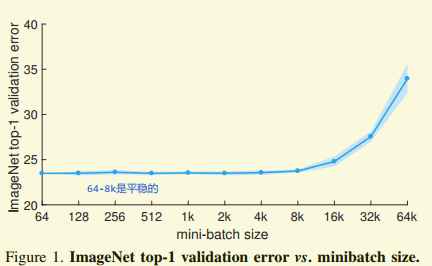
\includegraphics[width=.9\linewidth]{Accurate_Large_Minibatch_SGD.org_imgs/20201114_181812_yX0kcP.png}
\end{center}

如何在保证准确率的基础上进行分布式训练?
\section{Main Work}
\label{sec:org62bdd0b}
\begin{itemize}
\item 使用Linear Scaling Rule适应不同batch size的学习率
\item 采用warm-up方法逐渐提高学习率
\item Batch Normalization
\begin{itemize}
\item BN打破每个样本loss的独立性,这里的独立性不利于训练。使用BN后,单个样本的loss依赖所在batch的其他样本
\item 各个batch可以看做独立的样本,保持n不变,那么训练集中独立的样本个数不变。因此只改变batch size,loss不会受影响
\item 在整个训练集中,每个batch是独立的,假设总共有n个batch,如果n发生变化,则训练集的loss也会受到影响
\item 但是在分布式系统,单机为n,则整个系统为kn,kn可以看作k个batch,因此分布式不会对训练集的loss产生影响
\item 把n看做BN的超参数,只要固定n,则分布式训练就不会对系统的loss产生影响,文中n=32
\item 固定n,通过改变k实现mini-batch size的改变,通过这种方法,本文实现了分布式上训练达到与单机相同的训练效果
\end{itemize}
\item Communication
\begin{itemize}
\item binary blocks algorithm, 梯度的aggregation
\end{itemize}
\end{itemize}
\section{Innovation}
\label{sec:org4db980f}
在保证准确率的前提下进行分布式训练,对batch size 进行探讨。
\section{Summary}
\label{sec:org44f72ed}
\begin{itemize}
\item 行文十分流畅,从中学习到了分布式深度学习一些通用细节
\end{itemize}
\end{document}
